% Options for packages loaded elsewhere
\PassOptionsToPackage{unicode}{hyperref}
\PassOptionsToPackage{hyphens}{url}
\PassOptionsToPackage{dvipsnames,svgnames,x11names}{xcolor}
%
\documentclass[
  letterpaper,
  DIV=11,
  numbers=noendperiod]{scrartcl}

\usepackage{amsmath,amssymb}
\usepackage{iftex}
\ifPDFTeX
  \usepackage[T1]{fontenc}
  \usepackage[utf8]{inputenc}
  \usepackage{textcomp} % provide euro and other symbols
\else % if luatex or xetex
  \usepackage{unicode-math}
  \defaultfontfeatures{Scale=MatchLowercase}
  \defaultfontfeatures[\rmfamily]{Ligatures=TeX,Scale=1}
\fi
\usepackage{lmodern}
\ifPDFTeX\else  
    % xetex/luatex font selection
\fi
% Use upquote if available, for straight quotes in verbatim environments
\IfFileExists{upquote.sty}{\usepackage{upquote}}{}
\IfFileExists{microtype.sty}{% use microtype if available
  \usepackage[]{microtype}
  \UseMicrotypeSet[protrusion]{basicmath} % disable protrusion for tt fonts
}{}
\makeatletter
\@ifundefined{KOMAClassName}{% if non-KOMA class
  \IfFileExists{parskip.sty}{%
    \usepackage{parskip}
  }{% else
    \setlength{\parindent}{0pt}
    \setlength{\parskip}{6pt plus 2pt minus 1pt}}
}{% if KOMA class
  \KOMAoptions{parskip=half}}
\makeatother
\usepackage{xcolor}
\setlength{\emergencystretch}{3em} % prevent overfull lines
\setcounter{secnumdepth}{-\maxdimen} % remove section numbering
% Make \paragraph and \subparagraph free-standing
\makeatletter
\ifx\paragraph\undefined\else
  \let\oldparagraph\paragraph
  \renewcommand{\paragraph}{
    \@ifstar
      \xxxParagraphStar
      \xxxParagraphNoStar
  }
  \newcommand{\xxxParagraphStar}[1]{\oldparagraph*{#1}\mbox{}}
  \newcommand{\xxxParagraphNoStar}[1]{\oldparagraph{#1}\mbox{}}
\fi
\ifx\subparagraph\undefined\else
  \let\oldsubparagraph\subparagraph
  \renewcommand{\subparagraph}{
    \@ifstar
      \xxxSubParagraphStar
      \xxxSubParagraphNoStar
  }
  \newcommand{\xxxSubParagraphStar}[1]{\oldsubparagraph*{#1}\mbox{}}
  \newcommand{\xxxSubParagraphNoStar}[1]{\oldsubparagraph{#1}\mbox{}}
\fi
\makeatother

\usepackage{color}
\usepackage{fancyvrb}
\newcommand{\VerbBar}{|}
\newcommand{\VERB}{\Verb[commandchars=\\\{\}]}
\DefineVerbatimEnvironment{Highlighting}{Verbatim}{commandchars=\\\{\}}
% Add ',fontsize=\small' for more characters per line
\usepackage{framed}
\definecolor{shadecolor}{RGB}{241,243,245}
\newenvironment{Shaded}{\begin{snugshade}}{\end{snugshade}}
\newcommand{\AlertTok}[1]{\textcolor[rgb]{0.68,0.00,0.00}{#1}}
\newcommand{\AnnotationTok}[1]{\textcolor[rgb]{0.37,0.37,0.37}{#1}}
\newcommand{\AttributeTok}[1]{\textcolor[rgb]{0.40,0.45,0.13}{#1}}
\newcommand{\BaseNTok}[1]{\textcolor[rgb]{0.68,0.00,0.00}{#1}}
\newcommand{\BuiltInTok}[1]{\textcolor[rgb]{0.00,0.23,0.31}{#1}}
\newcommand{\CharTok}[1]{\textcolor[rgb]{0.13,0.47,0.30}{#1}}
\newcommand{\CommentTok}[1]{\textcolor[rgb]{0.37,0.37,0.37}{#1}}
\newcommand{\CommentVarTok}[1]{\textcolor[rgb]{0.37,0.37,0.37}{\textit{#1}}}
\newcommand{\ConstantTok}[1]{\textcolor[rgb]{0.56,0.35,0.01}{#1}}
\newcommand{\ControlFlowTok}[1]{\textcolor[rgb]{0.00,0.23,0.31}{\textbf{#1}}}
\newcommand{\DataTypeTok}[1]{\textcolor[rgb]{0.68,0.00,0.00}{#1}}
\newcommand{\DecValTok}[1]{\textcolor[rgb]{0.68,0.00,0.00}{#1}}
\newcommand{\DocumentationTok}[1]{\textcolor[rgb]{0.37,0.37,0.37}{\textit{#1}}}
\newcommand{\ErrorTok}[1]{\textcolor[rgb]{0.68,0.00,0.00}{#1}}
\newcommand{\ExtensionTok}[1]{\textcolor[rgb]{0.00,0.23,0.31}{#1}}
\newcommand{\FloatTok}[1]{\textcolor[rgb]{0.68,0.00,0.00}{#1}}
\newcommand{\FunctionTok}[1]{\textcolor[rgb]{0.28,0.35,0.67}{#1}}
\newcommand{\ImportTok}[1]{\textcolor[rgb]{0.00,0.46,0.62}{#1}}
\newcommand{\InformationTok}[1]{\textcolor[rgb]{0.37,0.37,0.37}{#1}}
\newcommand{\KeywordTok}[1]{\textcolor[rgb]{0.00,0.23,0.31}{\textbf{#1}}}
\newcommand{\NormalTok}[1]{\textcolor[rgb]{0.00,0.23,0.31}{#1}}
\newcommand{\OperatorTok}[1]{\textcolor[rgb]{0.37,0.37,0.37}{#1}}
\newcommand{\OtherTok}[1]{\textcolor[rgb]{0.00,0.23,0.31}{#1}}
\newcommand{\PreprocessorTok}[1]{\textcolor[rgb]{0.68,0.00,0.00}{#1}}
\newcommand{\RegionMarkerTok}[1]{\textcolor[rgb]{0.00,0.23,0.31}{#1}}
\newcommand{\SpecialCharTok}[1]{\textcolor[rgb]{0.37,0.37,0.37}{#1}}
\newcommand{\SpecialStringTok}[1]{\textcolor[rgb]{0.13,0.47,0.30}{#1}}
\newcommand{\StringTok}[1]{\textcolor[rgb]{0.13,0.47,0.30}{#1}}
\newcommand{\VariableTok}[1]{\textcolor[rgb]{0.07,0.07,0.07}{#1}}
\newcommand{\VerbatimStringTok}[1]{\textcolor[rgb]{0.13,0.47,0.30}{#1}}
\newcommand{\WarningTok}[1]{\textcolor[rgb]{0.37,0.37,0.37}{\textit{#1}}}

\providecommand{\tightlist}{%
  \setlength{\itemsep}{0pt}\setlength{\parskip}{0pt}}\usepackage{longtable,booktabs,array}
\usepackage{calc} % for calculating minipage widths
% Correct order of tables after \paragraph or \subparagraph
\usepackage{etoolbox}
\makeatletter
\patchcmd\longtable{\par}{\if@noskipsec\mbox{}\fi\par}{}{}
\makeatother
% Allow footnotes in longtable head/foot
\IfFileExists{footnotehyper.sty}{\usepackage{footnotehyper}}{\usepackage{footnote}}
\makesavenoteenv{longtable}
\usepackage{graphicx}
\makeatletter
\def\maxwidth{\ifdim\Gin@nat@width>\linewidth\linewidth\else\Gin@nat@width\fi}
\def\maxheight{\ifdim\Gin@nat@height>\textheight\textheight\else\Gin@nat@height\fi}
\makeatother
% Scale images if necessary, so that they will not overflow the page
% margins by default, and it is still possible to overwrite the defaults
% using explicit options in \includegraphics[width, height, ...]{}
\setkeys{Gin}{width=\maxwidth,height=\maxheight,keepaspectratio}
% Set default figure placement to htbp
\makeatletter
\def\fps@figure{htbp}
\makeatother

\KOMAoption{captions}{tableheading}
\makeatletter
\@ifpackageloaded{caption}{}{\usepackage{caption}}
\AtBeginDocument{%
\ifdefined\contentsname
  \renewcommand*\contentsname{Table of contents}
\else
  \newcommand\contentsname{Table of contents}
\fi
\ifdefined\listfigurename
  \renewcommand*\listfigurename{List of Figures}
\else
  \newcommand\listfigurename{List of Figures}
\fi
\ifdefined\listtablename
  \renewcommand*\listtablename{List of Tables}
\else
  \newcommand\listtablename{List of Tables}
\fi
\ifdefined\figurename
  \renewcommand*\figurename{}
\else
  \newcommand\figurename{}
\fi
\ifdefined\tablename
  \renewcommand*\tablename{Table}
\else
  \newcommand\tablename{Table}
\fi
}
\@ifpackageloaded{float}{}{\usepackage{float}}
\floatstyle{ruled}
\@ifundefined{c@chapter}{\newfloat{codelisting}{h}{lop}}{\newfloat{codelisting}{h}{lop}[chapter]}
\floatname{codelisting}{Listing}
\newcommand*\listoflistings{\listof{codelisting}{List of Listings}}
\makeatother
\makeatletter
\makeatother
\makeatletter
\@ifpackageloaded{caption}{}{\usepackage{caption}}
\@ifpackageloaded{subcaption}{}{\usepackage{subcaption}}
\makeatother

\ifLuaTeX
  \usepackage{selnolig}  % disable illegal ligatures
\fi
\usepackage{bookmark}

\IfFileExists{xurl.sty}{\usepackage{xurl}}{} % add URL line breaks if available
\urlstyle{same} % disable monospaced font for URLs
\hypersetup{
  colorlinks=true,
  linkcolor={blue},
  filecolor={Maroon},
  citecolor={Blue},
  urlcolor={Blue},
  pdfcreator={LaTeX via pandoc}}


\author{}
\date{}

\begin{document}


\subsection{Writing an academic paper with
Quarto}\label{sec-Quarto_exercise}

In this exercise we will start to write an academic manuscript using
Quarto and incorporating data from the example R project we have used in
the other exercises. The project is the same that is created in the
first workflow \href{@sec-Rproj_zenodo_exercise}{exercise}, however to
save time or in case you haven't completed this exercise we will start
with the finished output from it.

If you would prefer to view the exercise script offline, here is a PDF
version: Download exercise instructions

\subsubsection{Step 1: Download the
resources}\label{step-1-download-the-resources}

\begin{itemize}
\item
  Click here to download the resources for the exercise: Download
  resources for exercise
\item
  Unzip the downloaded file and move the folder to a location on your
  computer where you can easily find it.
\end{itemize}

\subsubsection{Step 2: Open the project in
RStudio}\label{step-2-open-the-project-in-rstudio}

\begin{itemize}
\tightlist
\item
  Open RStudio and navigate to the folder where you saved the resources
  for the exercise.
\item
  Open the Rstudio project file in the directory
  (\texttt{Rice\_farm\_analysis.Rproj})
\end{itemize}

\subsubsection{Step 3: Download Quarto}\label{step-3-download-quarto}

\begin{itemize}
\item
  \textbf{Note}: Because Quarto is bundled with Rstudio if you have a
  recent version of Rstudio you may already have Quarto installed. To
  check go to \emph{File \textgreater{} New File} and you should see
  \emph{Quarto} Document as an option.
\item
  If you do not have Quarto installed you can install it from the Quarto
  website \href{https://quarto.org/docs/download/}{here}
\end{itemize}

\subsubsection{Step 4: Create a Quarto document for the article
content}\label{step-4-create-a-quarto-document-for-the-article-content}

The Quarto website provides a
\href{https://github.com/quarto-ext/manuscript-template-rstudio}{template}
for creating a Manuscript project but we will create one from scratch so
that you understand the various files.

\begin{itemize}
\tightlist
\item
  The 1st step is to create a Quarto document that will act as the
  primary content file, go to \emph{File \textgreater{} New File
  \textgreater{} Quarto Document}. You don't need to add title or author
  information in the wizard as we will do this in the document itself.
\end{itemize}

\begin{figure}[H]

{\centering 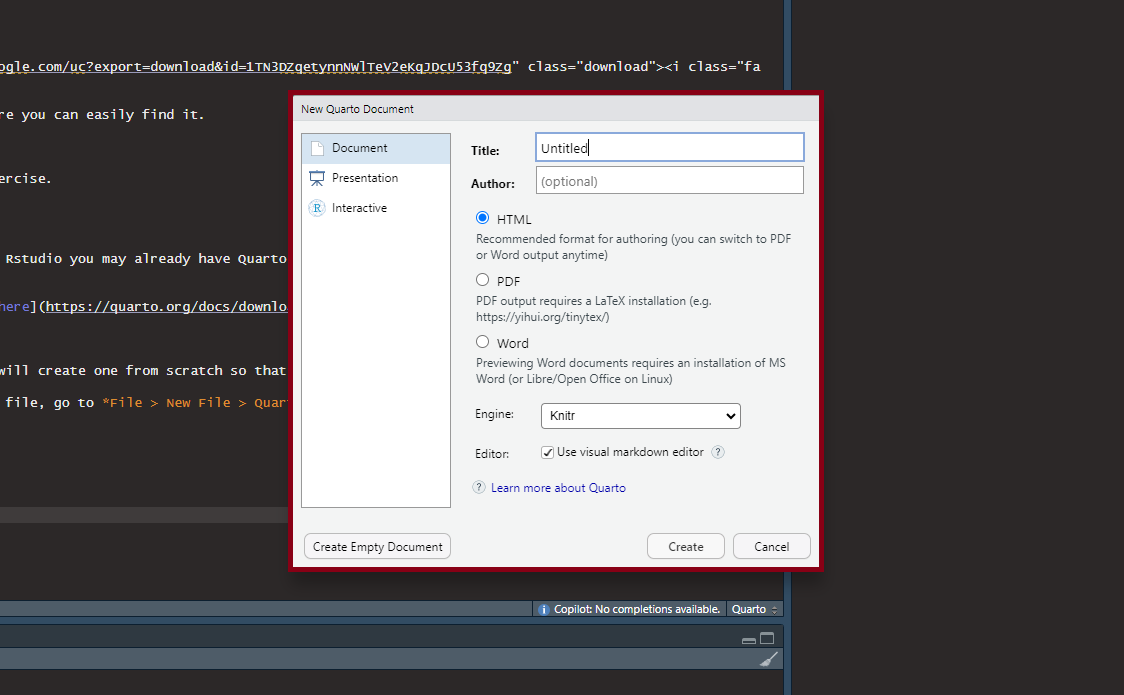
\includegraphics[width=0.7\textwidth,height=\textheight]{assets/images/quarto-new-file.png}

}

\caption{Quarto document wizard}

\end{figure}%

\begin{itemize}
\tightlist
\item
  Save the file as \texttt{index.qmd} in the root directory of the
  project. Using \texttt{index} as the file name is the convention for
  the main content file in a Quarto project and the software will look
  for this when attempting to create an output of the content. However
  it is possible to use a different file name if you prefer but it
  requires setting an option in the configuration file.
\end{itemize}

\subsubsection{\texorpdfstring{Step 5: Create a \texttt{\_quarto.yml}
configuration
file}{Step 5: Create a \_quarto.yml configuration file}}\label{step-5-create-a-_quarto.yml-configuration-file}

\href{https://en.wikipedia.org/wiki/YAML}{YAML} files (\texttt{.yml})
are configuration files, and in the case of Quarto the convention is to
use a file named \texttt{\_quarto.yml} in the root directory of the
project. This file will be used to set a range of options including the
project type, code execution options and options for the output
format/s.

\begin{itemize}
\tightlist
\item
  Create a new file with \emph{File \textgreater{} New File
  \textgreater{} Text File} and save it to the root directory of the
  project and name it \texttt{\_quarto.yml}. Adding the extension
  \texttt{.yml} will automatically set the file type to YAML.
\end{itemize}

\subsubsection{\texorpdfstring{Step 6: Specify the \texttt{Manuscript}
project type in the configuration
file}{Step 6: Specify the Manuscript project type in the configuration file}}\label{step-6-specify-the-manuscript-project-type-in-the-configuration-file}

\begin{itemize}
\item
  \textbf{Note}: All YAML options are set using
  \href{https://www.commonwl.org/user_guide/topics/yaml-guide.html\#key-value-pairs}{key-value
  pairs} and the Quarto documentation provides a
  \href{https://quarto.org/docs/projects/quarto-projects.html}{list of
  options} that can be set in the configuration file.
\item
  The first step is to identify your project as a manuscript by entering
  the following code in the \texttt{\_quarto.yml} file:
\end{itemize}

\begin{codelisting}

\caption{\texttt{\_quarto.yml}}

\begin{Shaded}
\begin{Highlighting}[]
\FunctionTok{project}\KeywordTok{:}\AttributeTok{ }
\AttributeTok{  }\FunctionTok{type}\KeywordTok{:}\AttributeTok{ manuscript}
\end{Highlighting}
\end{Shaded}

\end{codelisting}

\begin{itemize}
\tightlist
\item
  If you do want your main content file to be named something other than
  \texttt{index.*} you can add the file name with the \texttt{article}
  key (but make sure that your \texttt{.qmd} file name matches the
  entry):
\end{itemize}

\begin{codelisting}

\caption{\texttt{\_quarto.yml}}

\begin{Shaded}
\begin{Highlighting}[]
\FunctionTok{manuscript}\KeywordTok{:}
\AttributeTok{  }\FunctionTok{article}\KeywordTok{:}\AttributeTok{ Rice\_farm.qmd}
\end{Highlighting}
\end{Shaded}

\end{codelisting}

\subsubsection{Step 7: Set output formats in the configuration
file}\label{step-7-set-output-formats-in-the-configuration-file}

The next step is to set the output formats for the document. Quarto
supports outputting your manuscript to a range of formats simultaneously
including HTML, PDF, Docx and LaTeX. The output formats and their
individual options are also set in the \texttt{\_quarto.yml} file.

\begin{itemize}
\tightlist
\item
  For this exercise we will set the output formats to HTML, docx and
  PDF. Add the following code to the \texttt{\_quarto.yml} file:
\end{itemize}

\begin{codelisting}

\caption{\texttt{\_quarto.yml}}

\begin{Shaded}
\begin{Highlighting}[]
\FunctionTok{format}\KeywordTok{:}
\AttributeTok{  }\FunctionTok{html}\KeywordTok{:}
\AttributeTok{    }\FunctionTok{toc}\KeywordTok{:}\AttributeTok{ }\CharTok{true}
\AttributeTok{    }\FunctionTok{comments}\KeywordTok{:}
\AttributeTok{      }\FunctionTok{hypothesis}\KeywordTok{:}\AttributeTok{ }\CharTok{true}
\AttributeTok{  }\FunctionTok{docx}\KeywordTok{:}\AttributeTok{ default}
\end{Highlighting}
\end{Shaded}

\end{codelisting}

\begin{itemize}
\item
  For PDF outputs specifically, there a number of templates that have
  been produced to align with the formatting of major academic
  publishers. These are available as
  \href{https://quarto.org/docs/extensions/listing-journals.html}{Quarto
  extensions}.
\item
  For this exercise we will use the
  \href{https://github.com/quarto-journals/elsevier}{Elsevier template}.
  Quarto extensions can be installed directly using the terminal in
  Rstudio. To install the Elsevier template run the following code in
  the terminal: \texttt{quarto\ add\ quarto-journals/elsevier}
\end{itemize}

\begin{center}
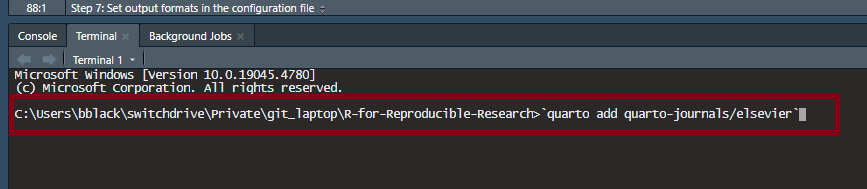
\includegraphics[width=0.7\textwidth,height=\textheight]{assets/images/quarto-elsevier-install.png}
\end{center}

\begin{itemize}
\tightlist
\item
  Once the template is installed you can set the PDF output to use the
  template by adding the following code to the \texttt{\_quarto.yml}
  file indented below the existing \texttt{format} entry:
\end{itemize}

\begin{codelisting}

\caption{\texttt{\_quarto.yml}}

\begin{Shaded}
\begin{Highlighting}[]
\AttributeTok{  }\FunctionTok{elsevier{-}pdf}\KeywordTok{:}\AttributeTok{ default}
\end{Highlighting}
\end{Shaded}

\end{codelisting}

\subsubsection{Step 8: Complete the front matter
content}\label{step-8-complete-the-front-matter-content}

The front matter of the document is where you can enter the title,
author/s and other metadata for the document. In the case of academic
manuscripts this also includes the abstract, keywords, author
institutions and roles (according to the
\href{https://authorservices.wiley.com/author-resources/Journal-Authors/open-access/credit.html}{CRediT
Taxonomy}). The full list of front matter options for Quarto manuscripts
can be found
\href{https://quarto.org/docs/authoring/front-matter.html}{here}.

Front matter is entered as YAML content at the start of the main content
file \texttt{index.qmd}. To be recognised as YAML content it must be
enclosed by three dashes \texttt{-\/-\/-} at the start and end of the
content block.

\begin{itemize}
\tightlist
\item
  Enter example front matter for this exercise as follows:
\end{itemize}

\begin{Shaded}
\begin{Highlighting}[]
\PreprocessorTok{{-}{-}{-}}
\FunctionTok{title}\KeywordTok{:}\AttributeTok{ An Analysis of Rice Production in Indonesia}
\FunctionTok{author}\KeywordTok{:}
\AttributeTok{  }\KeywordTok{{-}}\AttributeTok{ }\FunctionTok{name}\KeywordTok{:}\AttributeTok{ Jane Doe}
\AttributeTok{    }\FunctionTok{orcid}\KeywordTok{:}\AttributeTok{ 0000{-}0002{-}0760{-}5497}
\AttributeTok{    }\FunctionTok{corresponding}\KeywordTok{:}\AttributeTok{ }\CharTok{true}
\AttributeTok{    }\FunctionTok{email}\KeywordTok{:}\AttributeTok{ Janedoe@gmail.com}
\AttributeTok{    }\FunctionTok{roles}\KeywordTok{:}
\AttributeTok{      }\KeywordTok{{-}}\AttributeTok{ Investigation}
\AttributeTok{      }\KeywordTok{{-}}\AttributeTok{ Project administration}
\AttributeTok{      }\KeywordTok{{-}}\AttributeTok{ Software}
\AttributeTok{      }\KeywordTok{{-}}\AttributeTok{ Visualization}
\AttributeTok{    }\FunctionTok{affiliations}\KeywordTok{:}
\AttributeTok{      }\KeywordTok{{-}}\AttributeTok{ }\FunctionTok{id}\KeywordTok{:}\AttributeTok{ ETH\_PLUS}
\AttributeTok{        }\FunctionTok{name}\KeywordTok{:}\AttributeTok{ ETH Zürich}
\AttributeTok{        }\FunctionTok{department}\KeywordTok{:}\AttributeTok{ Planning of Landscape and Urban Systems (PLUS) Institut für Raum{-} und Landschaftsentwicklung (IRL)}
\AttributeTok{        }\FunctionTok{address}\KeywordTok{:}\AttributeTok{ HIL H 52.1, Stefano{-}Franscini{-}Platz 5}
\AttributeTok{        }\FunctionTok{city}\KeywordTok{:}\AttributeTok{ Zürich}
\AttributeTok{        }\FunctionTok{postal{-}code}\KeywordTok{:}\AttributeTok{ }\DecValTok{8093}
\AttributeTok{  }\KeywordTok{{-}}\AttributeTok{ }\FunctionTok{name}\KeywordTok{:}\AttributeTok{ John Doe}
\AttributeTok{    }\FunctionTok{orcid}\KeywordTok{:}\AttributeTok{ 0000{-}0002{-}7859{-}8394}
\AttributeTok{    }\FunctionTok{corresponding}\KeywordTok{:}\AttributeTok{ }\CharTok{false}
\AttributeTok{    }\FunctionTok{roles}\KeywordTok{:}\AttributeTok{ }\KeywordTok{[]}
\AttributeTok{    }\FunctionTok{affiliations}\KeywordTok{:}\AttributeTok{ }
\AttributeTok{      }\KeywordTok{{-}}\AttributeTok{ }\FunctionTok{id}\KeywordTok{:}\AttributeTok{ ETH\_PLUS}
\FunctionTok{keywords}\KeywordTok{:}
\AttributeTok{  }\KeywordTok{{-}}\AttributeTok{ Rice farms}
\AttributeTok{  }\KeywordTok{{-}}\AttributeTok{ Indonesia}
\AttributeTok{  }\KeywordTok{{-}}\AttributeTok{ Regional production}
\FunctionTok{abstract}\KeywordTok{: }\CharTok{|}
\NormalTok{  This is the abstract}
\FunctionTok{plain{-}language{-}summary}\KeywordTok{: }\CharTok{|}
\NormalTok{  Rice production data for the country of Indonesia is analysed ...}
\FunctionTok{date}\KeywordTok{:}\AttributeTok{ last{-}modified}
\FunctionTok{number{-}sections}\KeywordTok{:}\AttributeTok{ }\CharTok{true}
\PreprocessorTok{{-}{-}{-}}
\end{Highlighting}
\end{Shaded}

Now take some time to practice editing this content by, for example,
changing the title, adding yourself as an author or changing the
abstract. You will see that indentation is very important for YAML
content to work correctly.

One nice feature is the fact that you can use the
\texttt{affiliation:\ id} option to avoid needing to repeat details for
authors from the same institution.

\subsubsection{Step 7: Add manuscript
content}\label{step-7-add-manuscript-content}

Now we have our manuscript project and content file set up let's add
some content. Content in Quarto files is written in
\href{https://en.wikipedia.org/wiki/Markdown}{Markdown} format, which
takes some getting used to but will quickly become intuitive.

\begin{itemize}
\tightlist
\item
  Add some content to the \texttt{index.qmd} file. For example, use
  \texttt{\#} to create a heading and \texttt{\#\#} for subheadings:
\end{itemize}

\begin{Shaded}
\begin{Highlighting}[]
\FunctionTok{\# Introduction}

\NormalTok{Rice is a staple food in Indonesia and is grown in many regions across the country. The production of rice is a key economic activity in Indonesia and is a major source of employment for many people. In this study we analyse the production of different types of rice in different regions in Indonesia.  }

\FunctionTok{\# Methods}

\FunctionTok{\#\# Data}
\NormalTok{For this study we used data from the Indonesian Ministry of Agriculture on rice production in the country. The data was collected from different regions across Indonesia and includes information on the types of rice grown, the amount of rice produced and the area of land used for rice cultivation.}

\FunctionTok{\# Results}

\NormalTok{Figure 1 shows the distribution of rice production across different regions in Indonesia. Table 1 shows the types of rice grown in each region and the amount of rice produced.}
\end{Highlighting}
\end{Shaded}

Now lets render our manuscript for the first time to see how the output
looks. To render the document click the \texttt{Render} button in the
top of the Rstudio source pane:

\begin{center}
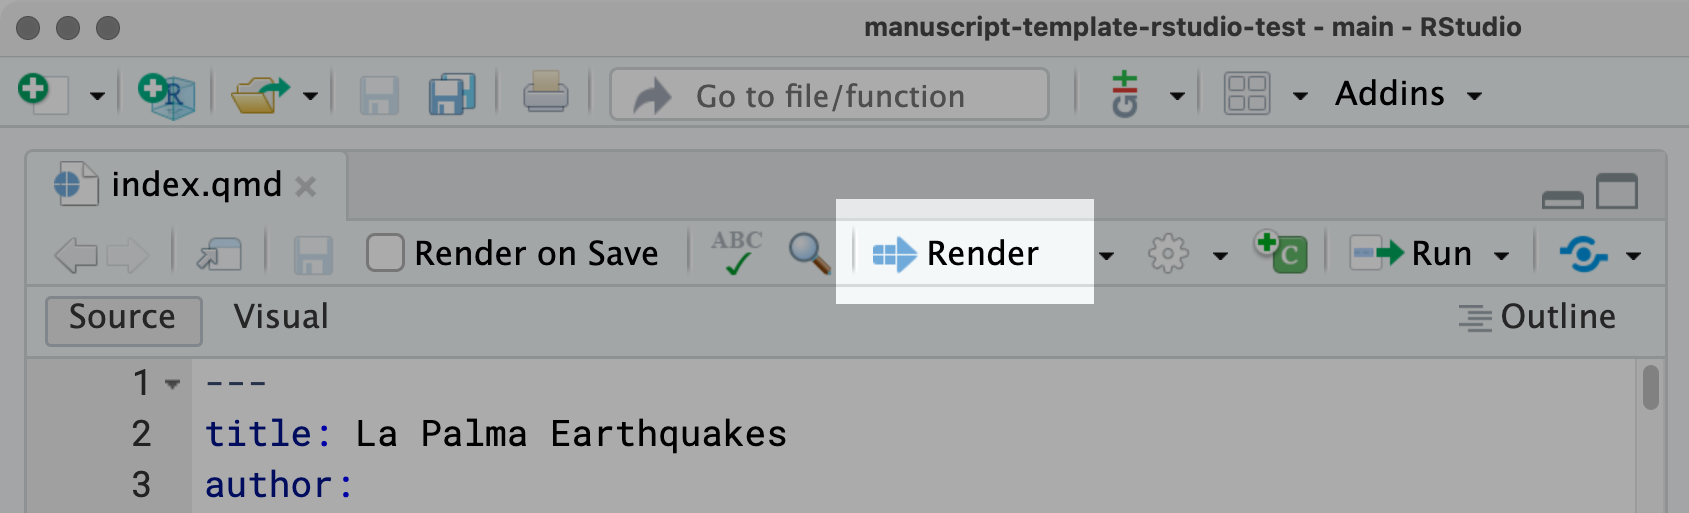
\includegraphics[width=0.7\textwidth,height=\textheight]{assets/images/rstudio-render-button.png}
\end{center}

This will render the document to HTML and open it in the viewer pane on
the right:

\begin{center}
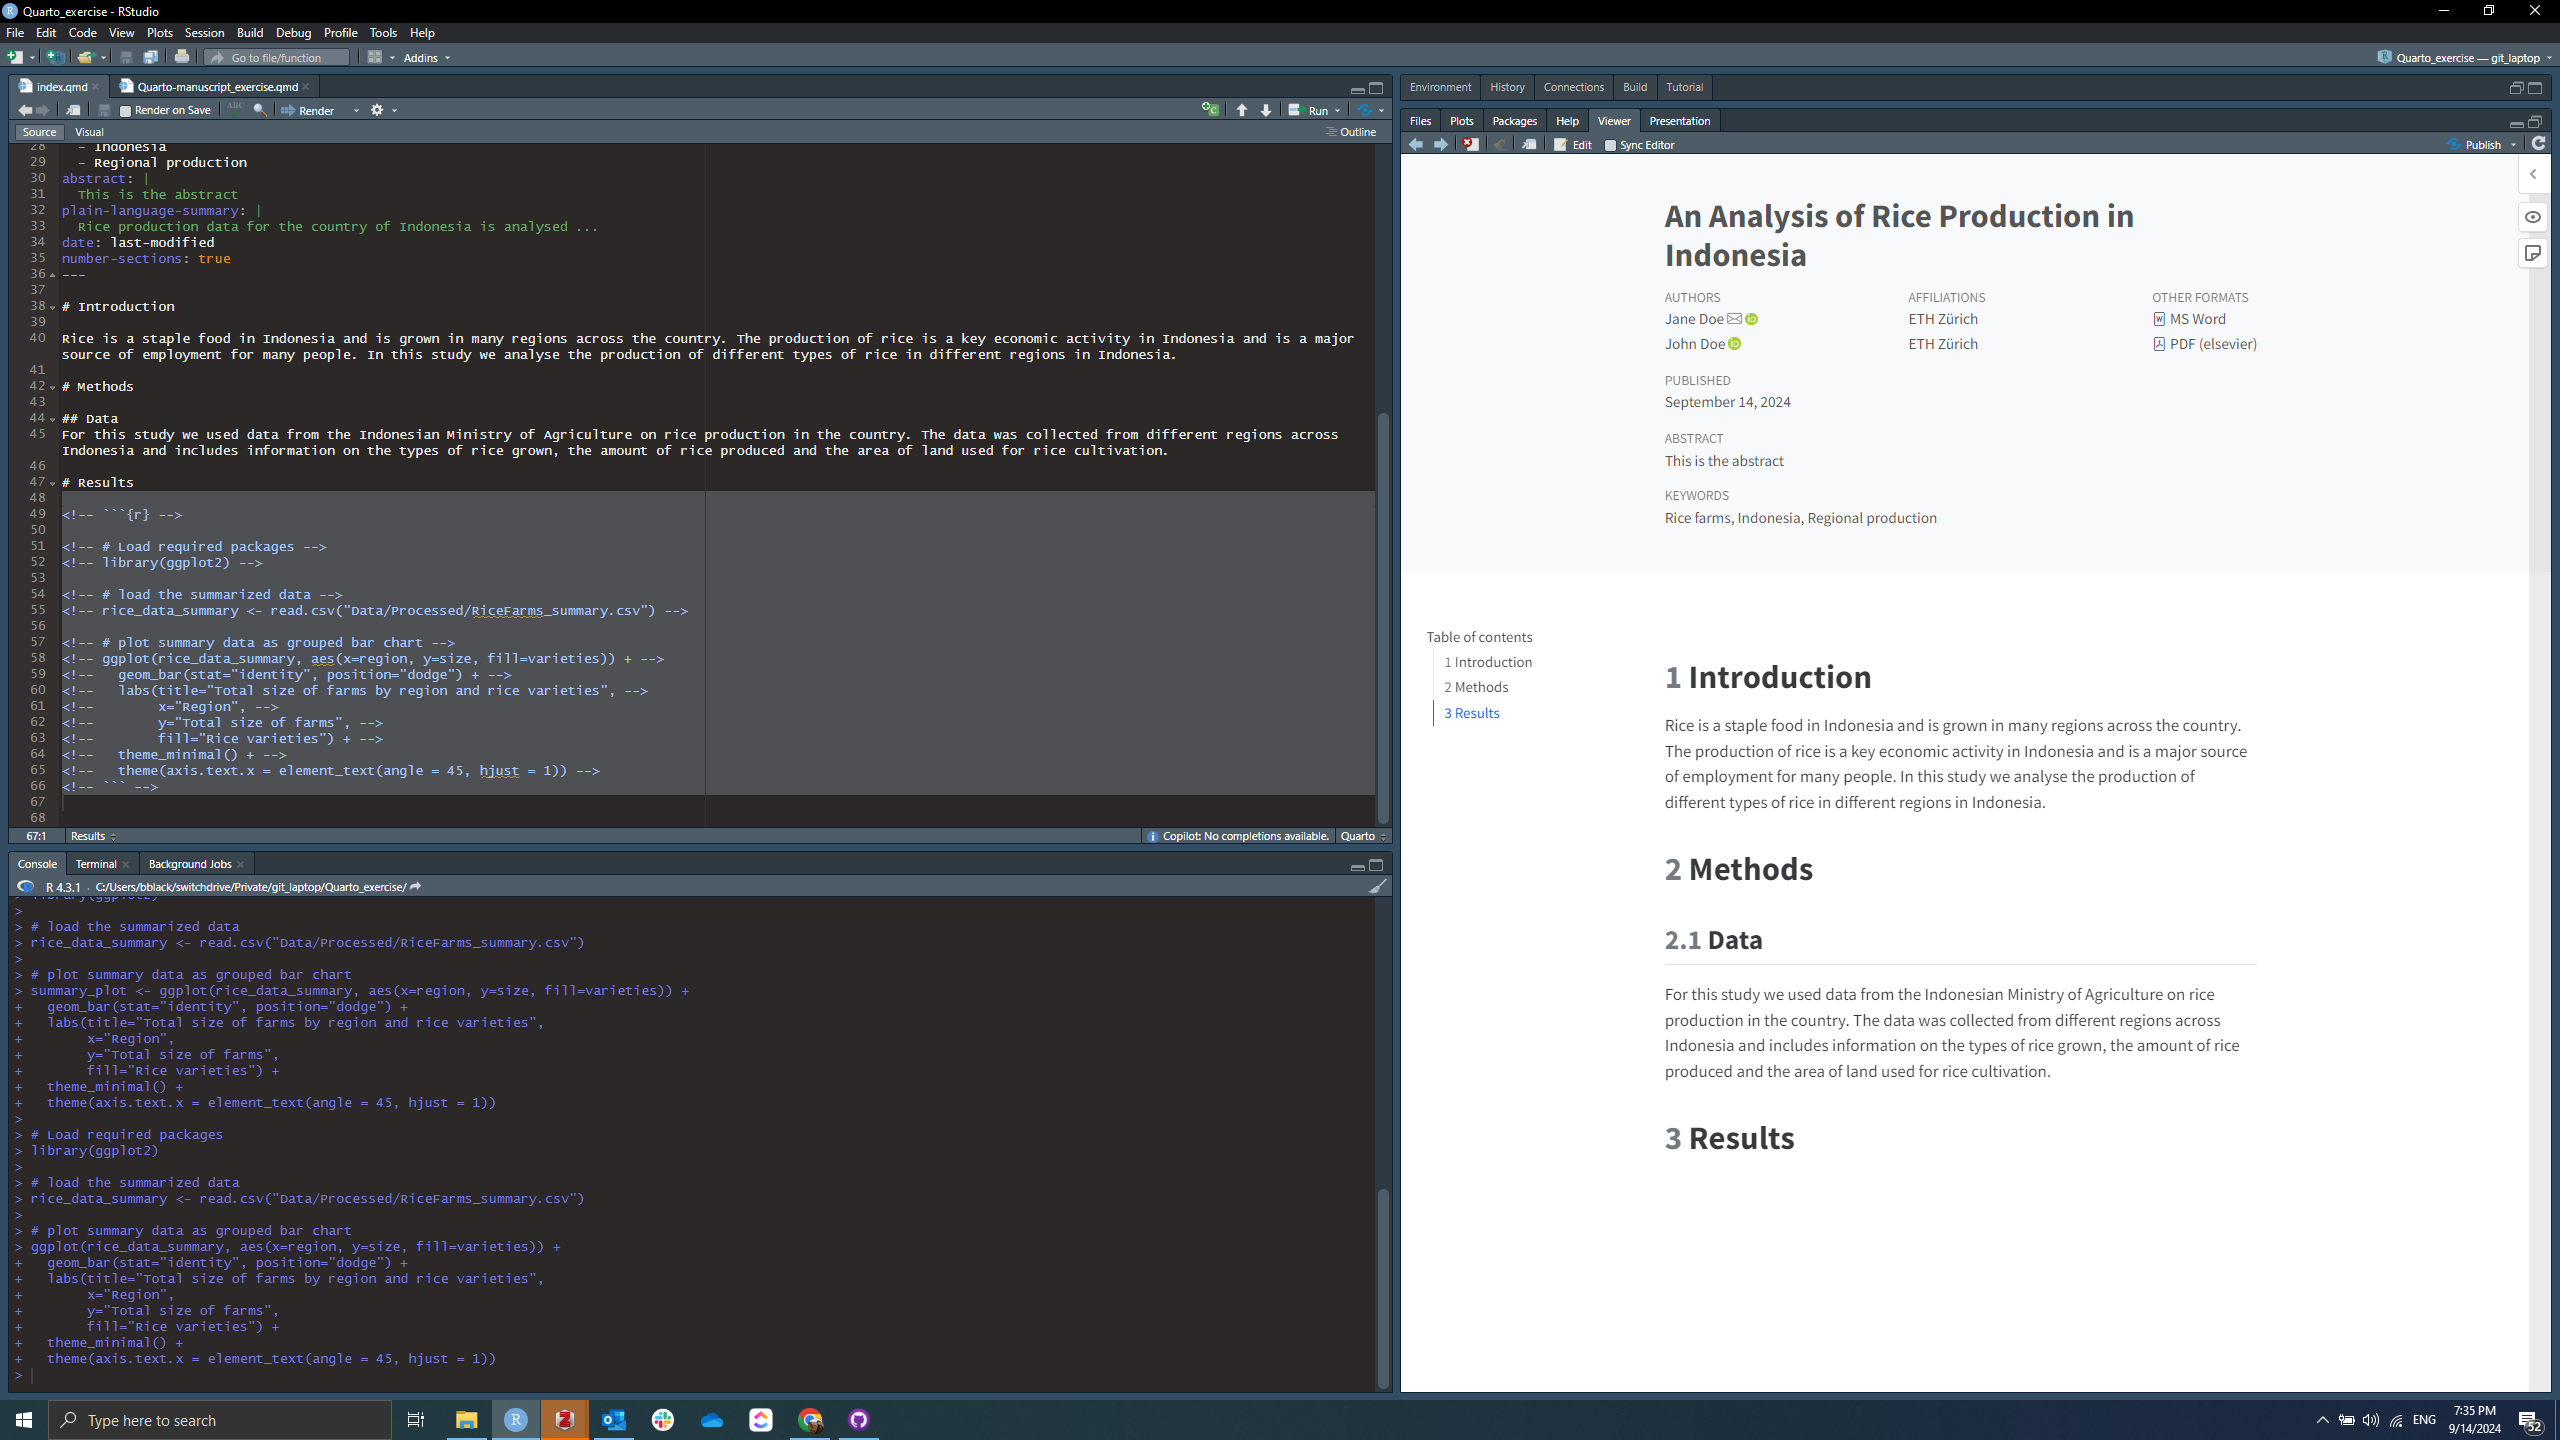
\includegraphics[width=0.7\textwidth,height=\textheight]{assets/images/quarto-html-output.png}
\end{center}

\subsubsection{Step 8: Add Figures and
Tables}\label{step-8-add-figures-and-tables}

Figures and tables can be added to quarto documents using code blocks in
various programming languages. To add a code block into a Quarto
document you use three backticks followed by the language name in
braces, for example an R chunk would be:
\texttt{\textasciigrave{}\textasciigrave{}\textasciigrave{}\{r\}} and
then close the block with another three backticks. Code blocks are
executed when the document is rendered and the output is included in the
final document (although this behaviour can be controlled with
\href{https://quarto.org/docs/computations/execution-options.html}{execution
options}).

Lets add a figure to the document using the R code from the exercise
script \texttt{Scripts/02\_data\_visualisation.R} to create a bar chart
of the area of farms growing different types in different regions in
Indonesia.

\begin{itemize}
\tightlist
\item
  Add the following code block to the \texttt{index.qmd} file below the
  \texttt{Results} heading:
  31b8e172-b470-440e-83d8-e6b185028602:dAB5AHAAZQA6AE8AUQBCAGoAQQBHAEkAQQBOAHcAQQA1AEEARwBVAEEATgBnAEIAagBBAEMAMABBAE8AQQBBADQAQQBEAGcAQQBaAEEAQQB0AEEARABRAEEAWQBRAEEAdwBBAEcAVQBBAEwAUQBBADUAQQBHAE0AQQBPAFEAQgBpAEEAQwAwAEEAWgBnAEIAbQBBAEQAWQBBAE4AdwBCAGoAQQBHAFEAQQBOAEEAQQB3AEEARABRAEEAWgBRAEEAMgBBAEQAQQBBAAoAcABvAHMAaQB0AGkAbwBuADoATQBRAEEAdwBBAEQASQBBAE4AZwBBAHcAQQBBAD0APQAKAHAAcgBlAGYAaQB4ADoACgBzAG8AdQByAGMAZQA6AFkAQQBCAGcAQQBHAEEAQQBlAHcAQgA3AEEASABJAEEAZgBRAEIAOQBBAEEAbwBBAEkAdwBBAGcAQQBFAHcAQQBiAHcAQgBoAEEARwBRAEEASQBBAEIAeQBBAEcAVQBBAGMAUQBCADEAQQBHAGsAQQBjAGcAQgBsAEEARwBRAEEASQBBAEIAdwBBAEcARQBBAFkAdwBCAHIAQQBHAEUAQQBaAHcAQgBsAEEASABNAEEAQwBnAEIAcwBBAEcAawBBAFkAZwBCAHkAQQBHAEUAQQBjAGcAQgA1AEEAQwBnAEEAWgB3AEIAbgBBAEgAQQBBAGIAQQBCAHYAQQBIAFEAQQBNAGcAQQBwAEEAQQBvAEEAQwBnAEEAagBBAEMAQQBBAGIAQQBCAHYAQQBHAEUAQQBaAEEAQQBnAEEASABRAEEAYQBBAEIAbABBAEMAQQBBAGMAdwBCADEAQQBHADAAQQBiAFEAQgBoAEEASABJAEEAYQBRAEIANgBBAEcAVQBBAFoAQQBBAGcAQQBHAFEAQQBZAFEAQgAwAEEARwBFAEEAQwBnAEIAeQBBAEcAawBBAFkAdwBCAGwAQQBGADgAQQBaAEEAQgBoAEEASABRAEEAWQBRAEIAZgBBAEgATQBBAGQAUQBCAHQAQQBHADAAQQBZAFEAQgB5AEEASABrAEEASQBBAEEAOABBAEMAMABBAEkAQQBCAHkAQQBHAFUAQQBZAFEAQgBrAEEAQwA0AEEAWQB3AEIAegBBAEgAWQBBAEsAQQBBAGkAQQBFAFEAQQBZAFEAQgAwAEEARwBFAEEATAB3AEIAUQBBAEgASQBBAGIAdwBCAGoAQQBHAFUAQQBjAHcAQgB6AEEARwBVAEEAWgBBAEEAdgBBAEYASQBBAGEAUQBCAGoAQQBHAFUAQQBSAGcAQgBoAEEASABJAEEAYgBRAEIAegBBAEYAOABBAGMAdwBCADEAQQBHADAAQQBiAFEAQgBoAEEASABJAEEAZQBRAEEAdQBBAEcATQBBAGMAdwBCADIAQQBDAEkAQQBLAFEAQQBLAEEAQQBvAEEASQB3AEEAZwBBAEgAQQBBAGIAQQBCAHYAQQBIAFEAQQBJAEEAQgB6AEEASABVAEEAYgBRAEIAdABBAEcARQBBAGMAZwBCADUAQQBDAEEAQQBaAEEAQgBoAEEASABRAEEAWQBRAEEAZwBBAEcARQBBAGMAdwBBAGcAQQBHAGMAQQBjAGcAQgB2AEEASABVAEEAYwBBAEIAbABBAEcAUQBBAEkAQQBCAGkAQQBHAEUAQQBjAGcAQQBnAEEARwBNAEEAYQBBAEIAaABBAEgASQBBAGQAQQBBAEsAQQBHAGMAQQBaAHcAQgB3AEEARwB3AEEAYgB3AEIAMABBAEMAZwBBAGMAZwBCAHAAQQBHAE0AQQBaAFEAQgBmAEEARwBRAEEAWQBRAEIAMABBAEcARQBBAFgAdwBCAHoAQQBIAFUAQQBiAFEAQgB0AEEARwBFAEEAYwBnAEIANQBBAEMAdwBBAEkAQQBCAGgAQQBHAFUAQQBjAHcAQQBvAEEASABnAEEAUABRAEIAeQBBAEcAVQBBAFoAdwBCAHAAQQBHADgAQQBiAGcAQQBzAEEAQwBBAEEAZQBRAEEAOQBBAEgATQBBAGEAUQBCADYAQQBHAFUAQQBMAEEAQQBnAEEARwBZAEEAYQBRAEIAcwBBAEcAdwBBAFAAUQBCADIAQQBHAEUAQQBjAGcAQgBwAEEARwBVAEEAZABBAEIAcABBAEcAVQBBAGMAdwBBAHAAQQBDAGsAQQBJAEEAQQByAEEAQQBvAEEASQBBAEEAZwBBAEcAYwBBAFoAUQBCAHYAQQBHADAAQQBYAHcAQgBpAEEARwBFAEEAYwBnAEEAbwBBAEgATQBBAGQAQQBCAGgAQQBIAFEAQQBQAFEAQQBpAEEARwBrAEEAWgBBAEIAbABBAEcANABBAGQAQQBCAHAAQQBIAFEAQQBlAFEAQQBpAEEAQwB3AEEASQBBAEIAdwBBAEcAOABBAGMAdwBCAHAAQQBIAFEAQQBhAFEAQgB2AEEARwA0AEEAUABRAEEAaQBBAEcAUQBBAGIAdwBCAGsAQQBHAGMAQQBaAFEAQQBpAEEAQwBrAEEASQBBAEEAcgBBAEEAbwBBAEkAQQBBAGcAQQBHAHcAQQBZAFEAQgBpAEEASABNAEEASwBBAEIAMABBAEcAawBBAGQAQQBCAHMAQQBHAFUAQQBQAFEAQQBpAEEARgBRAEEAYgB3AEIAMABBAEcARQBBAGIAQQBBAGcAQQBIAE0AQQBhAFEAQgA2AEEARwBVAEEASQBBAEIAdgBBAEcAWQBBAEkAQQBCAG0AQQBHAEUAQQBjAGcAQgB0AEEASABNAEEASQBBAEIAaQBBAEgAawBBAEkAQQBCAHkAQQBHAFUAQQBaAHcAQgBwAEEARwA4AEEAYgBnAEEAZwBBAEcARQBBAGIAZwBCAGsAQQBDAEEAQQBjAGcAQgBwAEEARwBNAEEAWgBRAEEAZwBBAEgAWQBBAFkAUQBCAHkAQQBHAGsAQQBaAFEAQgAwAEEARwBrAEEAWgBRAEIAegBBAEMASQBBAEwAQQBBAEsAQQBDAEEAQQBJAEEAQQBnAEEAQwBBAEEASQBBAEEAZwBBAEMAQQBBAGUAQQBBADkAQQBDAEkAQQBVAGcAQgBsAEEARwBjAEEAYQBRAEIAdgBBAEcANABBAEkAZwBBAHMAQQBBAG8AQQBJAEEAQQBnAEEAQwBBAEEASQBBAEEAZwBBAEMAQQBBAEkAQQBCADUAQQBEADAAQQBJAGcAQgBVAEEARwA4AEEAZABBAEIAaABBAEcAdwBBAEkAQQBCAHoAQQBHAGsAQQBlAGcAQgBsAEEAQwBBAEEAYgB3AEIAbQBBAEMAQQBBAFoAZwBCAGgAQQBIAEkAQQBiAFEAQgB6AEEAQwBJAEEATABBAEEASwBBAEMAQQBBAEkAQQBBAGcAQQBDAEEAQQBJAEEAQQBnAEEAQwBBAEEAWgBnAEIAcABBAEcAdwBBAGIAQQBBADkAQQBDAEkAQQBVAGcAQgBwAEEARwBNAEEAWgBRAEEAZwBBAEgAWQBBAFkAUQBCAHkAQQBHAGsAQQBaAFEAQgAwAEEARwBrAEEAWgBRAEIAegBBAEMASQBBAEsAUQBBAGcAQQBDAHMAQQBDAGcAQQBnAEEAQwBBAEEAZABBAEIAbwBBAEcAVQBBAGIAUQBCAGwAQQBGADgAQQBiAFEAQgBwAEEARwA0AEEAYQBRAEIAdABBAEcARQBBAGIAQQBBAG8AQQBDAGsAQQBJAEEAQQByAEEAQQBvAEEASQBBAEEAZwBBAEgAUQBBAGEAQQBCAGwAQQBHADAAQQBaAFEAQQBvAEEARwBFAEEAZQBBAEIAcABBAEgATQBBAEwAZwBCADAAQQBHAFUAQQBlAEEAQgAwAEEAQwA0AEEAZQBBAEEAZwBBAEQAMABBAEkAQQBCAGwAQQBHAHcAQQBaAFEAQgB0AEEARwBVAEEAYgBnAEIAMABBAEYAOABBAGQAQQBCAGwAQQBIAGcAQQBkAEEAQQBvAEEARwBFAEEAYgBnAEIAbgBBAEcAdwBBAFoAUQBBAGcAQQBEADAAQQBJAEEAQQAwAEEARABVAEEATABBAEEAZwBBAEcAZwBBAGEAZwBCADEAQQBIAE0AQQBkAEEAQQBnAEEARAAwAEEASQBBAEEAeABBAEMAawBBAEsAUQBBAEsAQQBHAEEAQQBZAEEAQgBnAEEAQQA9AD0ACgBzAHUAZgBmAGkAeAA6AA==:31b8e172-b470-440e-83d8-e6b185028602
\end{itemize}

Now if you re-render the document you should see the figure included in
the output.

\subsubsection{Step 9: Add
Cross-references}\label{step-9-add-cross-references}

Quarto allows you to
\href{https://quarto.org/docs/authoring/cross-references.html}{cross-reference}
figures, tables and sections in your document.

\begin{itemize}
\tightlist
\item
  Add a label to the figure code block by adding the following line at
  the top of the code block:
\end{itemize}

\begin{Shaded}
\begin{Highlighting}[]
\InformationTok{\textasciigrave{}\textasciigrave{}\textasciigrave{}\{r\}}
\InformationTok{\#| label: fig{-}barchart}
\InformationTok{\textasciigrave{}\textasciigrave{}\textasciigrave{}}
\end{Highlighting}
\end{Shaded}

\begin{itemize}
\tightlist
\item
  Now add a cross-reference to this figure in the text by changing the
  word \texttt{Figure\ 1} to \texttt{@fig-barchart} in the 1st sentence
  of the \texttt{Results} section:
\end{itemize}

\begin{Shaded}
\begin{Highlighting}[]
\FunctionTok{\# Results}

\NormalTok{@fig{-}barchart shows the distribution of rice production across different regions in Indonesia. Table 1 shows the types of rice grown in each region and the amount of rice produced.}
\end{Highlighting}
\end{Shaded}

\begin{itemize}
\tightlist
\item
  Now if you re-render the document you will see that the figure has
  been automatically numbered and the text now contains a hyperlinked
  cross reference to the figure:
\end{itemize}

\begin{center}
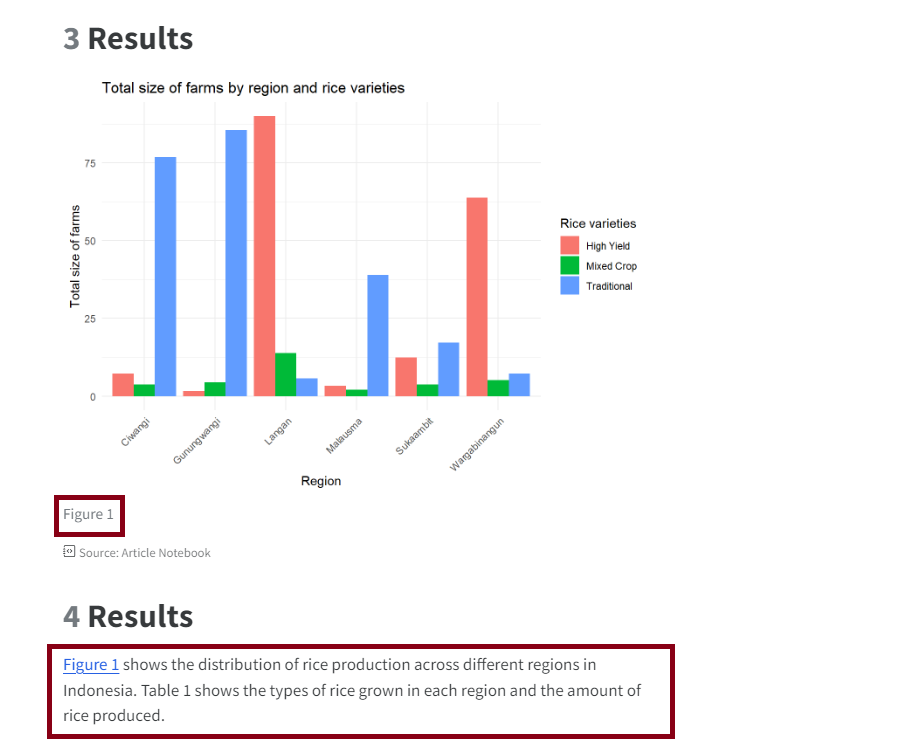
\includegraphics[width=0.7\textwidth,height=\textheight]{assets/images/quarto-figure-cross-reference.png}
\end{center}

\subsubsection{Step 10: Add citations}\label{step-10-add-citations}

Quarto provides the functionality to not only add citations to your
documents but to automatically generate a bibliography, both of which
can be formatted according to a wide range of citation styles to meet
journal requirements. For a detailed explanation of citations with
Quarto see the guide
\href{https://quarto.org/docs/authoring/citations.html}{here}.

Quarto uses the standard Pandoc markdown representation for citations,
whereby citations go inside square brackets and are separated by
semicolons, e.g.~\texttt{{[}@citation{]}}. Citations can be entered
manually however they need to have a corresponding entry in the articles
bibliography file (a \texttt{.bib} or \texttt{.csl} file in the root
directory of the project). Instead, we will add a citation using the
wizard in the \href{https://quarto.org/docs/visual-editor/}{Quarto
visual editor} which will automatically create the citation entry in the
bibliography file.

\begin{itemize}
\tightlist
\item
  At the top of the source pane click the \texttt{Visual} button to
  switch to the visual editor:
\end{itemize}

\begin{center}
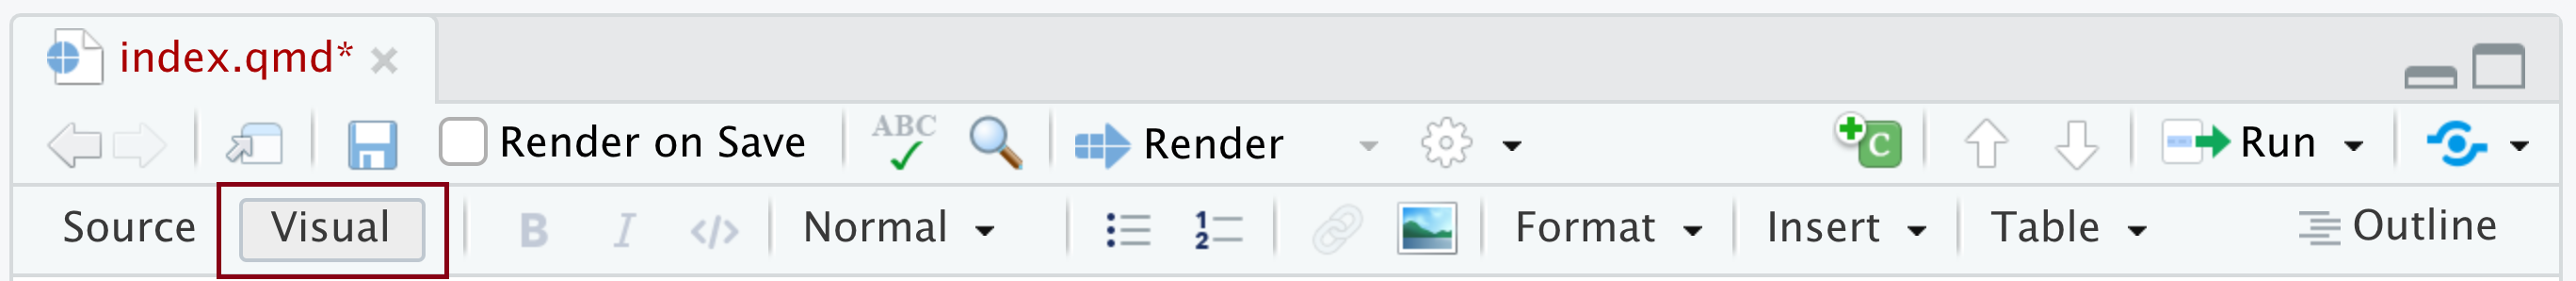
\includegraphics[width=0.7\textwidth,height=\textheight]{assets/images/visual-editing-switch-modes.png}
\end{center}

\begin{itemize}
\tightlist
\item
  Navigate the methods section and position the cursor at the end of the
  sentence:
\end{itemize}

\begin{Shaded}
\begin{Highlighting}[]
\NormalTok{For this study we used data from the Indonesian Ministry of Agriculture on rice production in the country.}
\end{Highlighting}
\end{Shaded}

\begin{itemize}
\tightlist
\item
  In the Visual editor tool bar at the top the top of the source pane
  click \emph{Insert} and in the drop down menu select \emph{Citation}
  (or alternatively use the keyboard shortcut \emph{Ctrl + Shift + F8}
  on windows). This will open the \textbf{Insert Citation} wizard:
\end{itemize}

\begin{center}
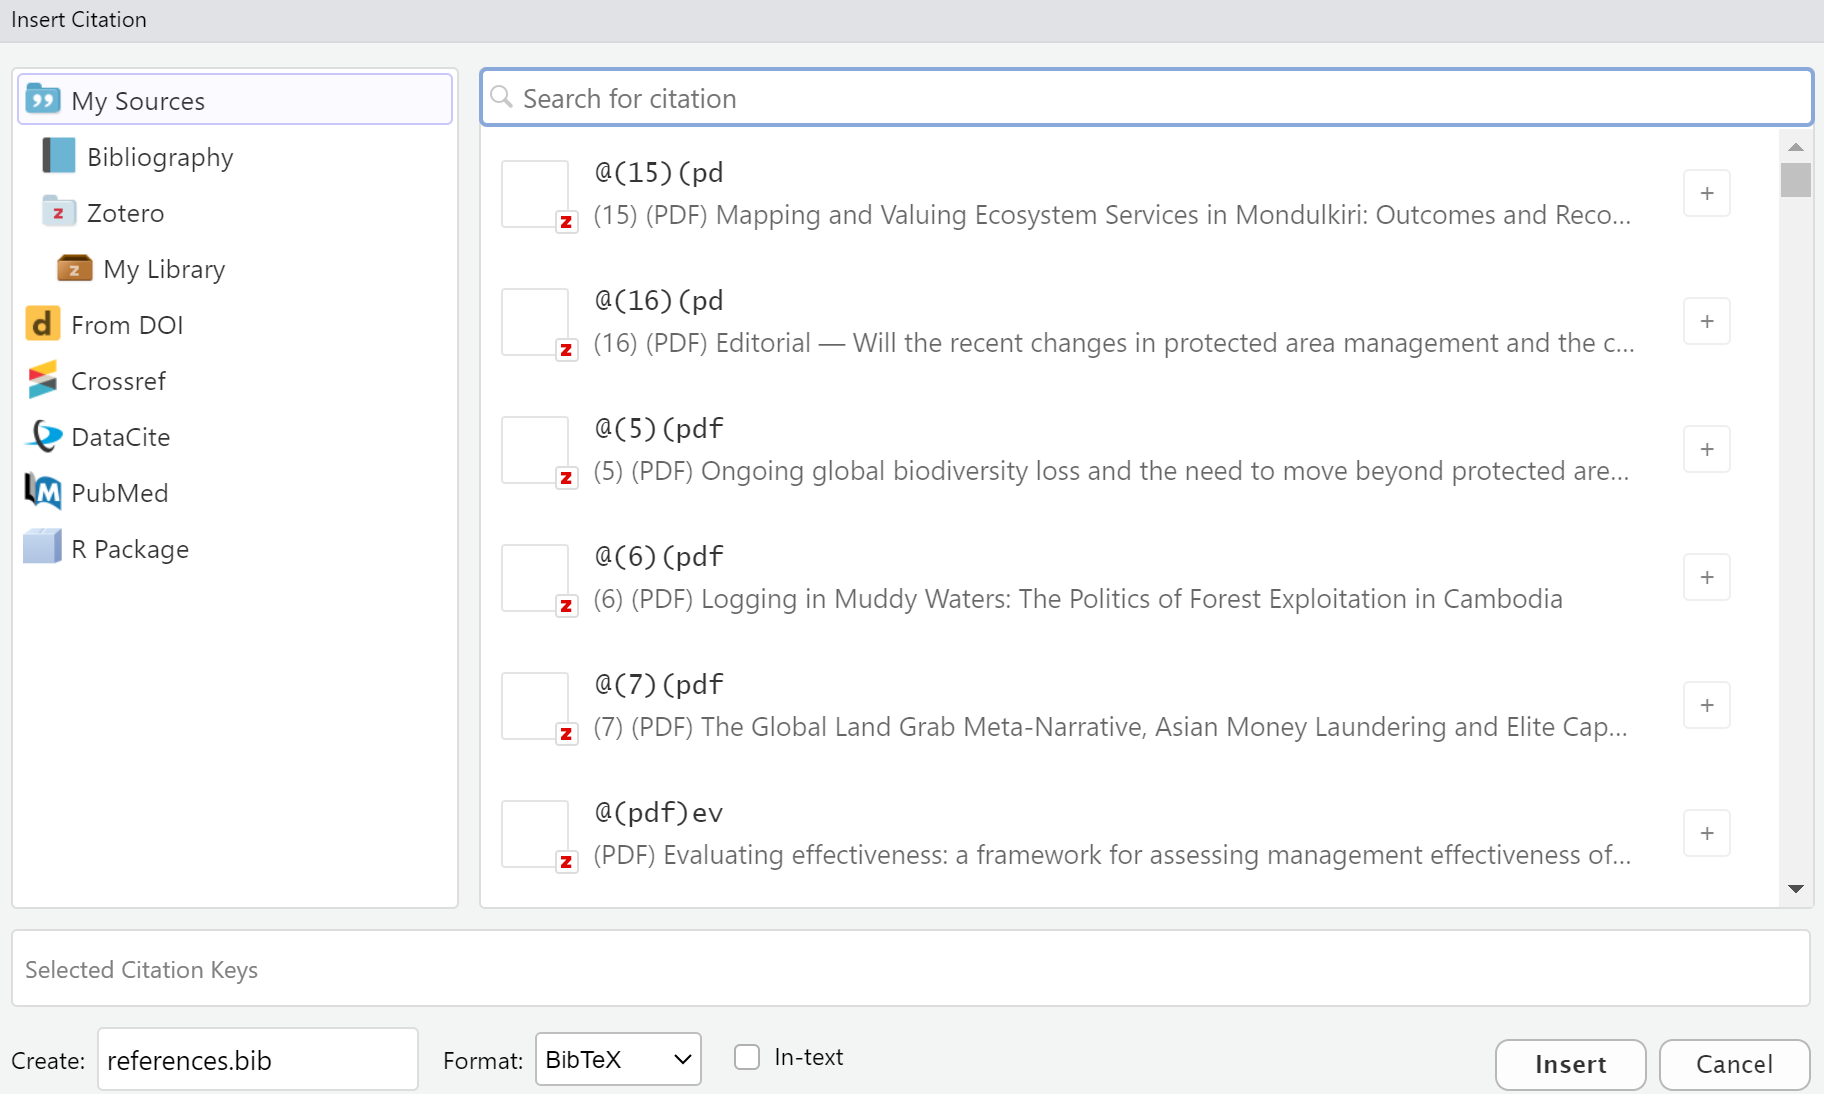
\includegraphics[width=0.7\textwidth,height=\textheight]{assets/images/insert_citation.png}
\end{center}

\begin{itemize}
\tightlist
\item
  The Rice Farms data used for the exercises comes from the
  \href{https://rdrr.io/rforge/plm/man/RiceFarms.html}{\texttt{plm}}
  package so we will cite this as an example (even though it is totally
  accurate in terms of the sentence content). Click on the tab for R
  packages on the left side of the wizard, enter \textbf{plm} in the
  search bar and click on the entry in the window below to select it:
\end{itemize}

\begin{center}
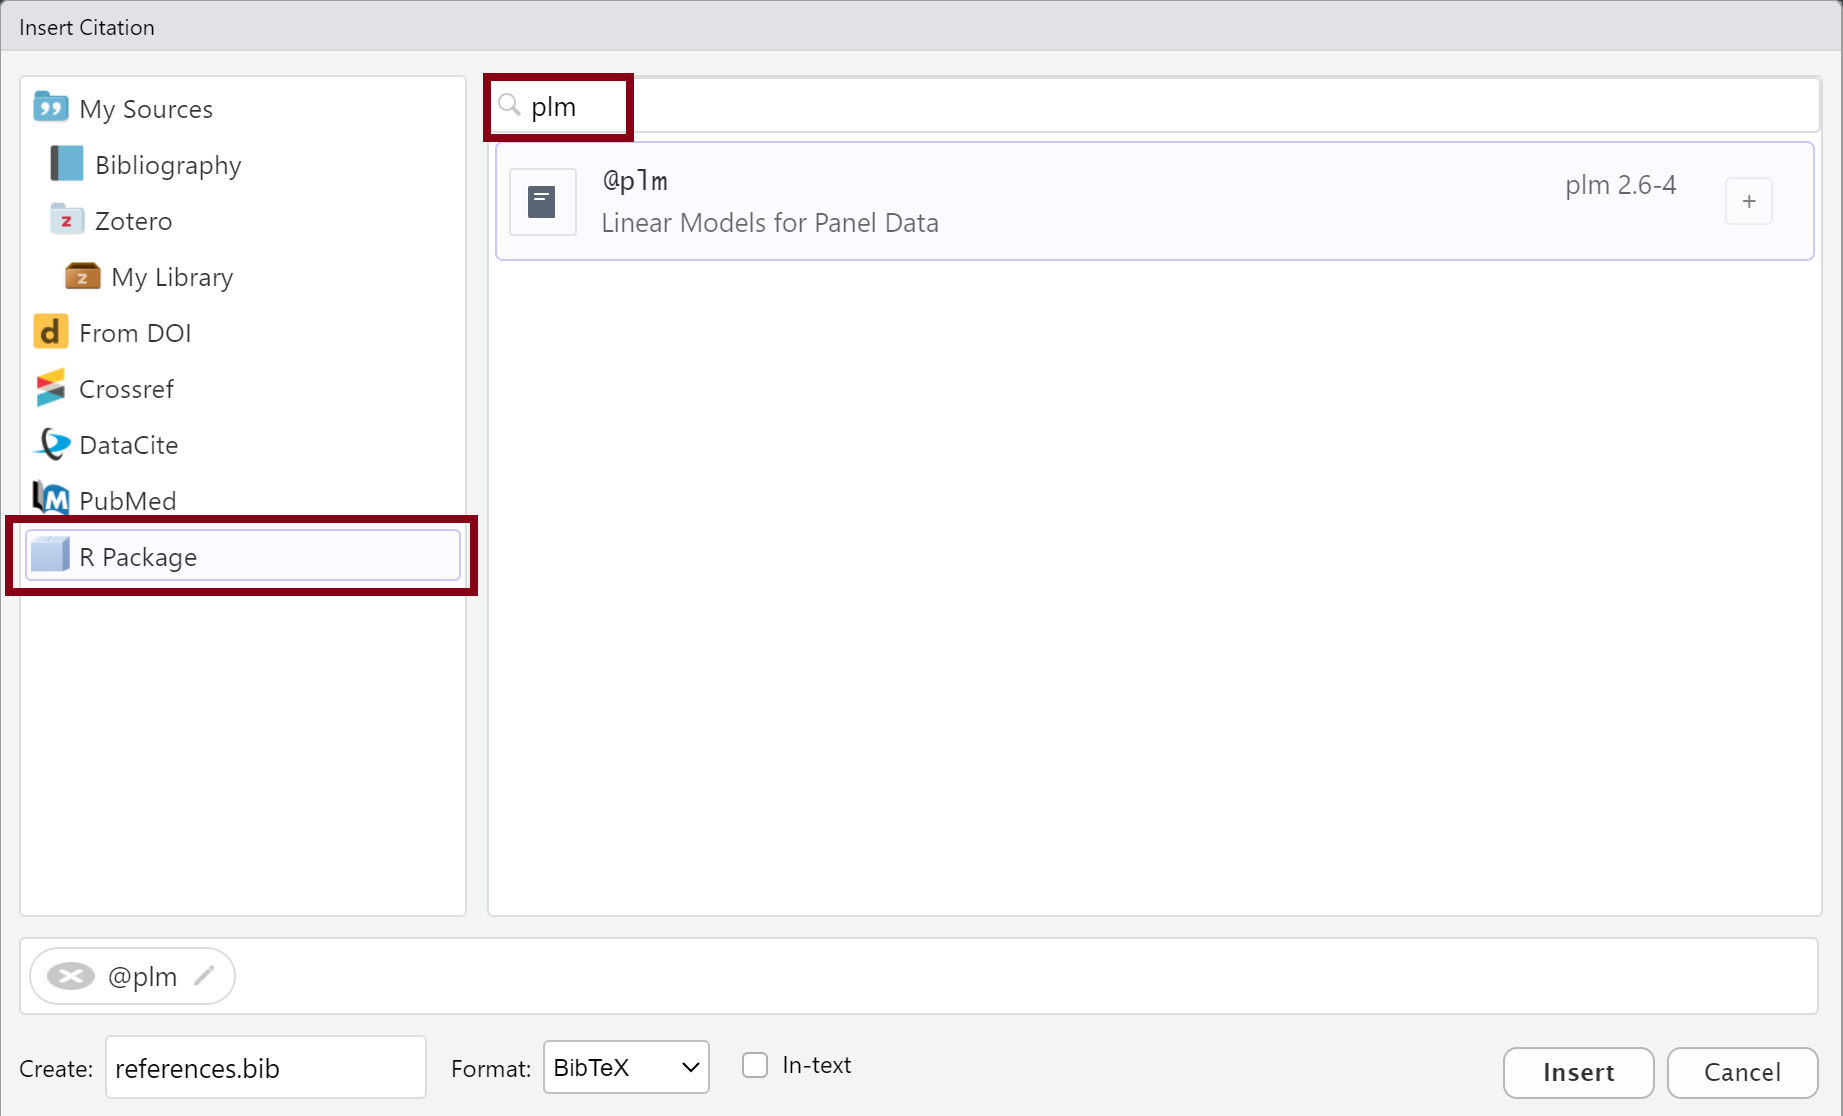
\includegraphics[width=0.7\textwidth,height=\textheight]{assets/images/cite-plm.png}
\end{center}

\begin{itemize}
\item
  Make sure the \textbf{Create} box in the bottom left corner of the
  wizard has a value in it, the default should be
  \texttt{references.bib}.
\item
  Now click \textbf{Insert} and the wizard will close, you will see that
  the citation has been added at the cursor location and a
  \texttt{references.bib} has been created in the root directory of the
  project. If you openthis file you can see the bibliographic details of
  the citation (Note if you have previously added citations or already
  created a \texttt{references.bib} file citations will all be added to
  the same file.
\end{itemize}

Now when you render the document this citation will automatically be
hyperlinked to the corresponding entry in the bibliography that is
appended to the end of the document.

\textbf{Tip:} In our experience the easiest method of adding academic
citations is to use the
\href{https://quarto.org/docs/visual-editor/technical.html\#citations-from-zotero}{Quarto-Zotero}
integration. In this case you select the Zotero tab in the
\textbf{Insert Citation} wizard and if Zotero is running on your
computer you will be able to search your whole library to add citations.

\subsubsection{Summary}\label{summary}

In this exercise we have only touched upon a few of the many of the
useful features of Quarto for writing reproducible research documents.
As such we would urge you to look through the
\href{https://quarto.org/docs/guide/}{Quarto documentation} to learn
about some of the other features as well as useful packages and
extensions such as the
\href{https://claudiozandonella.github.io/trackdown/}{trackdown} package
which allows you to convert Quarto documents in Google docs (and back to
Quarto again) to facilitate collaboration with users not familiar with
the format.



<script type="application/javascript" src="light-dark.js"></script>


\end{document}
